\PassOptionsToPackage{usenames, dvipsnames}{xcolor}
\documentclass[11pt,aspectratio=169,t]{beamer}

\usepackage[utf8]{inputenc}

\usetheme{UNIPD}
% First one is logo in title slide (we recommend use a horizontal image), and second one is the logo used in the remaining slides (we recommend use a square image)
\setLogos{lib/logos/dei_white.png}{lib/logos/dei_white_vertical.png} 

\usepackage{listings}
\usepackage[listings]{tcolorbox}

\usepackage{pgfplots}
\pgfplotsset{compat=1.3}
\tikzset{pointille/.style={dash pattern = on 2pt off 2pt on 6pt off 2pt}}
\tikzset{points/.style={dash pattern = on 1pt off 1pt}}
\tikzset{tirets/.style={dash pattern = on 5pt off 5pt}}

%\renewcommand{\only}{}

\usetikzlibrary{positioning}
\tikzset{>=stealth}
\newcommand{\tikzmark}[3][]{\tikz[remember picture,baseline] \node [anchor=base,#1](#2){$#3$};}
\usetikzlibrary{automata}

\usepackage{booktabs} 
\usepackage{bm}
\usepackage{subcaption}
\usepackage{mathrsfs}

\usepackage{palatino}

\usepackage{scrextend}
\usepackage{wrapfig}

\usepackage{quiver}
%--------------------------------------- Drawings
\usepackage{tikz}
\usetikzlibrary{calc,decorations.pathmorphing,patterns}
\pgfdeclaredecoration{penciline}{initial}{
    \state{initial}[width=+\pgfdecoratedinputsegmentremainingdistance,
    auto corner on length=1mm,]{
        \pgfpathcurveto%
        {% From
            \pgfqpoint{\pgfdecoratedinputsegmentremainingdistance}
                      {\pgfdecorationsegmentamplitude}
        }
        {%  Control 1
        \pgfmathrand
        \pgfpointadd{\pgfqpoint{\pgfdecoratedinputsegmentremainingdistance}{0pt}}
                    {\pgfqpoint{-\pgfdecorationsegmentaspect
                     \pgfdecoratedinputsegmentremainingdistance}%
                               {\pgfmathresult\pgfdecorationsegmentamplitude}
                    }
        }
        {%TO 
        \pgfpointadd{\pgfpointdecoratedinputsegmentlast}{\pgfpoint{1pt}{1pt}}
        }
    }
    \state{final}{}
}

%-------------------------------------------------------

\graphicspath{ {./imgs/}}

\usepackage[backend=bibtex, style=ieee]{biblatex}
\addbibresource{ref.bib}
\nocite{*}
\renewcommand*{\bibfont}{\tiny}

\newcommand\numberthis{\addtocounter{equation}{1}\tag{\theequation}}

%-------------------------------------theorems--------------
\newtheorem*{conjecture}{Conjecture}
\newtheorem{ex}{Example}
\newtheorem{exercise}{Exercise}
\newtheorem{lem}{Lemma}
\newtheorem{proposition}{Proposition}
\newtheorem{thm}{Theorem}
\newtheorem{cor}{Corollary}
\newtheorem*{remark}{Remark}
\newtheorem*{defi}{Definition}
\theoremstyle{definition}
\newtheorem*{assumption}{Assumption}
\newtheorem{prob}{Switching control problem}

\setbeamertemplate{theorems}[numbered]
\setbeamertemplate{caption}[numbered]

%-------------------------------------------------------------%
%----------------------- Primary Definitions -----------------%

% This command set the default Color, is also possible to choose a custom color
\setPrimaryColor{UNIPDred} 

\definecolor{simpleBlack}{HTML}{202020}

\definecolor{c1}{HTML}{7FB069}
\definecolor{c2}{HTML}{A3E7FC}
\definecolor{c3}{HTML}{FB8B24}
\definecolor{c4}{HTML}{335C67}
\definecolor{c5}{HTML}{1B9AAA}
\definecolor{c7}{HTML}{4B4E6D}
\definecolor{c6}{HTML}{F38D68}
\definecolor{c8}{HTML}{F5D547}
\definecolor{c9}{RGB}{231,237,57}
\definecolor{c10}{RGB}{237,57,71}
\definecolor{c11}{RGB}{119,237,57}
\definecolor{c12}{RGB}{0,63,225}
\definecolor{c13}{RGB}{237,57,223}


\newcommand{\ket}[1]{\left| #1 \right>}
\newcommand{\bra}[1]{\left< #1 \right|}
\newcommand{\norm}[1]{\left|\left| #1 \right|\right|}
\newcommand{\inner}[2]{\left< #1,#2 \right>}
\newcommand{\Outer}[2]{ \left|#1\right>\left<#2\right| }
\newcommand{\expect}[1]{\left< #1 \right>}
\newcommand{\blue}{\color{blue}}
\newcommand{\red}[1]{{\color{red} #1}}
\newcommand{\virg}[1]{\lq\lq#1\ignorespacesafterend\rq\rq}

\newcommand{\tr}{{\rm tr}}
\newcommand{\diag}{{\rm diag}}
\newcommand{\Span}{{\rm span}}
\newcommand{\cl}{{\rm cl}}
\DeclareMathOperator{\rank}{rank}
\newcommand{\spec}{{\rm spec}}
\newcommand{\idem}{ {\rm idem}}
\newcommand{\res}{{\rm res}}
\newcommand{\supp}{{\rm supp}}
\newcommand{\lind}{\mathcal{L}}
\newcommand{\one}{\bm 1}
\newcommand{\zero}{\bm 0}
\newcommand{\alg}{{\rm alg}}
\newcommand{\img}{{\rm Im}}

\renewcommand{\H}{\mathcal{H}}
\renewcommand{\P}{\mathbb{P}}
\newcommand{\BH}{\mathcal{B}(\H)}
\newcommand{\hH}{\mathfrak{h}(\H)}
\renewcommand{\DH}{\mathfrak{D}(\H)}
\newcommand{\Piso}{\mathcal{P}}

\newcommand{\Prob}{{\mathbb{P}}} % Probability measure in the Algebraic framework
\newcommand{\E}{{\mathbb{E}}} % Expectation in the algebraic framework
\newcommand{\str}[1]{{[{\bm #1}]}}
\newcommand{\chr}[1]{#1}

\newcommand{\R}{\mathcal{R}}
\newcommand{\NR}{\mathcal{N^R}}
\newcommand{\Oo}{\mathcal{O}}
\newcommand{\NO}{\mathcal{N^O}}
\newcommand{\p}{\bar{\bm p}}

\newcommand{\pO}{\p\wedge\Oo}
\newcommand{\pNR}{\p\wedge\NR}
\newcommand{\pNO}{\p^{-1}\wedge\NO}
\newcommand{\pR}{\p^{-1}\wedge\R}
\newcommand{\X}{\mathbb{R}^n}
\newcommand{\A}{\mathscr{A}}
\newcommand{\pA}{\p\wedge\A}

%%% ------------------------------ code snippets

\definecolor{dot1}{HTML}{FF5F55}
\definecolor{dot2}{HTML}{FFBE2A}
\definecolor{dot3}{HTML}{22CA3D}

\definecolor{background}{RGB}{39, 40, 34}
\definecolor{string}{RGB}{230, 219, 116}
\definecolor{comment}{HTML}{489038}
\definecolor{normal}{RGB}{248, 248, 242}
\definecolor{identifier}{RGB}{166, 226, 46}

\lstdefinestyle{mystyle}{
    language=Matlab,                			% choose the language of the code
  numbers=left,                   		% where to put the line-numbers
  stepnumber=1,                   		% the step between two line-numbers. 
  lineskip=-5pt,
  numbersep=5pt,                  		% how far the line-numbers are from the code
  numberstyle=\tiny\color{string}\ttfamily,
  %backgroundcolor=\color{background},  		% choose the background color. You must add \usepackage{color}
  showspaces=false,               		% show spaces adding particular underscores
  showstringspaces=false,         		% underline spaces within strings
  showtabs=false,                 		% show tabs within strings adding particular underscores
  tabsize=4,                      		% sets default tabsize to 2 spaces
  captionpos=b,                   		% sets the caption-position to bottom
  breaklines=true,                		% sets automatic line breaking
  breakatwhitespace=true,         		% sets if automatic breaks should only happen at whitespace
  %title=\lstname,                 		% show the filename of files included with \lstinputlisting;
  basicstyle=\small\color{normal}\ttfamily,					% sets font style for the code
  keywordstyle=\small\color{magenta}\ttfamily,	% sets color for keywords
  stringstyle=\small\color{string}\ttfamily,		% sets color for strings
  commentstyle=\small\color{comment}\ttfamily,	% sets color for comments
  emph={format_string, eff_ana_bf, permute, eff_ana_btr},
  emphstyle=\color{identifier}\ttfamily, 
  aboveskip=0pt
}

\lstset{style=mystyle}

% First one is logo in title slide (we recommend use a horizontal image), and second one is the logo used in the remaining slides (we recommend use a square image)
\setLogos{lib/logos/dei_white.png}{lib/logos/dei_white_vertical.png} 

\newtcbox{\codebox}[1]{colback=white!5!simpleBlack,
colframe=simpleBlack,fonttitle=\bfseries, top= 0mm, drop fuzzy shadow, enhanced, hbox,
title={\hspace{-0.3cm}{\color{dot1} $\bullet$} {\color{dot2} $\bullet$} {\color{dot3} $\bullet\quad$} #1}}


\newcommand{\codesection}[2]{
\codebox{#1}{\vspace{-0.3cm}{\lstinputlisting[language=Matlab]{#2}}}}

\tcbuselibrary{skins}

\newtcblisting{code}[1]{listing only, 
colback=white!5!simpleBlack,
colframe=simpleBlack,
fonttitle=\bfseries, 
listing options = {style = mystyle},
top= 2mm,
drop fuzzy shadow, enhanced, hbox,
title={\hspace{-0.3cm}
{\color{dot1} $\bullet$} 
{\color{dot2} $\bullet$}
{\color{dot3} $\bullet\quad$} #1}}



\begin{document}

\title{Beamer presentation template}

\author{Tommaso Grigoletto}

\date{\today}
%-------------------------------------------TITLE CARD-------------------------------------
\setBGColor{UNIPDred}
\frame[noframenumbering]{\titlepage}

%-------------------------------------------INTRO----------------------------------------

\setLayout{vertical}
\begin{frame}[noframenumbering,plain]{Agenda}
	\vfill
	\centering
	    \textbf{\color{c1}  Introduction}\\ \bigskip
		\textbf{\color{c2}  System representation}\\ \bigskip
		\textbf{\color{c3}  System analysis}\\ \bigskip
		\textbf{\color{c4}  Control design}\\ \bigskip
	\vfill
\end{frame}

\setBGColor{c1}
\setLayout{horizontal}
\begin{frame}[noframenumbering,plain]{Overlay curvy arrows}
	\vfill
        \begin{equation*}
            \begin{cases}
                \rho(t+1) = \tikzmark{A}{\mathcal{A}}[\tikzmark{rho}{\rho(t)}]\\
                \tikzmark{p}{\bm{p}(t)} = \tikzmark{C}{\mathcal{C}}[\rho(t)]
            \end{cases}
        \end{equation*}
        \begin{tikzpicture}[overlay, remember picture,node distance =.8cm]
            \only<1->{
            \node[rectangle, fill=none, draw=red!20, thick,
            minimum width = 0.8cm, 
            minimum height = 0.6cm] (rhobox) at (rho) {};
            \node[,text width=8cm] (rhodescr) [above right =of rho]{$\rho$ are density operators:\\ $\rho\in\mathbb{C}^{n\times n}$, $\rho=\rho^\dag\geq0$ and $\tr[\rho]=1$\\
            \alert{Quantum probability distributions}};
            \draw[red!30,->,thick] (rhodescr) to [in=90,out=-90] (rho);}
        
            \only<1->{
            \node[rectangle, fill=none, draw=blue!30, thick,
            minimum width = 0.6cm, 
            minimum height = 0.5cm] (rhobox) at (A) {};
            \node[,text width=6cm] (Adescr) [above left=of A]{$\mathcal{A}$ is a linear completely positive and trace preserving map\\
            \alert{``Stochastic'' map}};
            \draw[blue!30,->,thick] (Adescr) to [in=90,out=-90] (A.north);}
            
            \only<2->{
            \node[rectangle, fill=none, draw=purple!30, thick,
            minimum width = 0.5cm, 
            minimum height = 0.5cm] (rhobox) at (C) {};
            \node[,text width=8cm] (Cdescr) [below right =of C]{$\mathcal{C}$ is a linear map that gives the probabilities of the outcome of a measurement \\
            \alert{Oputput map}};
            \draw[purple!30,->,thick] (Cdescr) to [in=-90,out=90] (C.south);}
            
            \only<2->{
            \node[rectangle, fill=none, draw=ForestGreen!30, thick,
            minimum width = 0.8cm, 
            minimum height = 0.6cm] (rhobox) at (p) {};
            \node[,xshift=1cm,text width=5cm] (pdescr) [below left =of p]{$\bm p$ are probability vectors:\\ $\bm p\in\mathbb{R}^m$ $\bm p_i\geq0$ and  $\sum_i\bm p_i = 1$\\
            \alert{Classical probability\\ distribution}};
            \draw[ForestGreen!30,->,thick] (pdescr) to [in=-135,out=90] (p.south);}
            
            \only<2->{ 
            \node[yshift=0.5cm,text width=10cm] (modeldescr) [below =of Cdescr]{\small{This model includes hidden markov model \\ but \textbf{does not include} the effects of conditioning. }};
            }
        \end{tikzpicture}
	\vfill
\end{frame}

\setLayout{vertical}
\begin{frame}{Sample frame title}
    
    In this slide, some important text will be
    \alert{highlighted} because it's important. Please, don't abuse it.
    
    \begin{block}{Remark}
        Sample text
    \end{block}
    
    \begin{alertblock}{Important theorem}
        Sample text in alert box
    \end{alertblock}
    
    \begin{examples}
        Sample text in green box. The title of the block is ``Examples".
    \end{examples}
    
\end{frame}

\setLayout{vertical}
\begin{frame}[noframenumbering,plain]{Optimal reduction}
	\vfill
	
		
	\begin{remark}	 
	 A first draft on the related ``Model reduction for Hidden Markov Models'' can be found on \tikzmark[UNIPDred]{link}{arXiv:2208.05968}
	\end{remark}
	\begin{tikzpicture}[overlay, remember picture,node distance =.8cm]
	    \node[](qr) at (-6,-1.5) {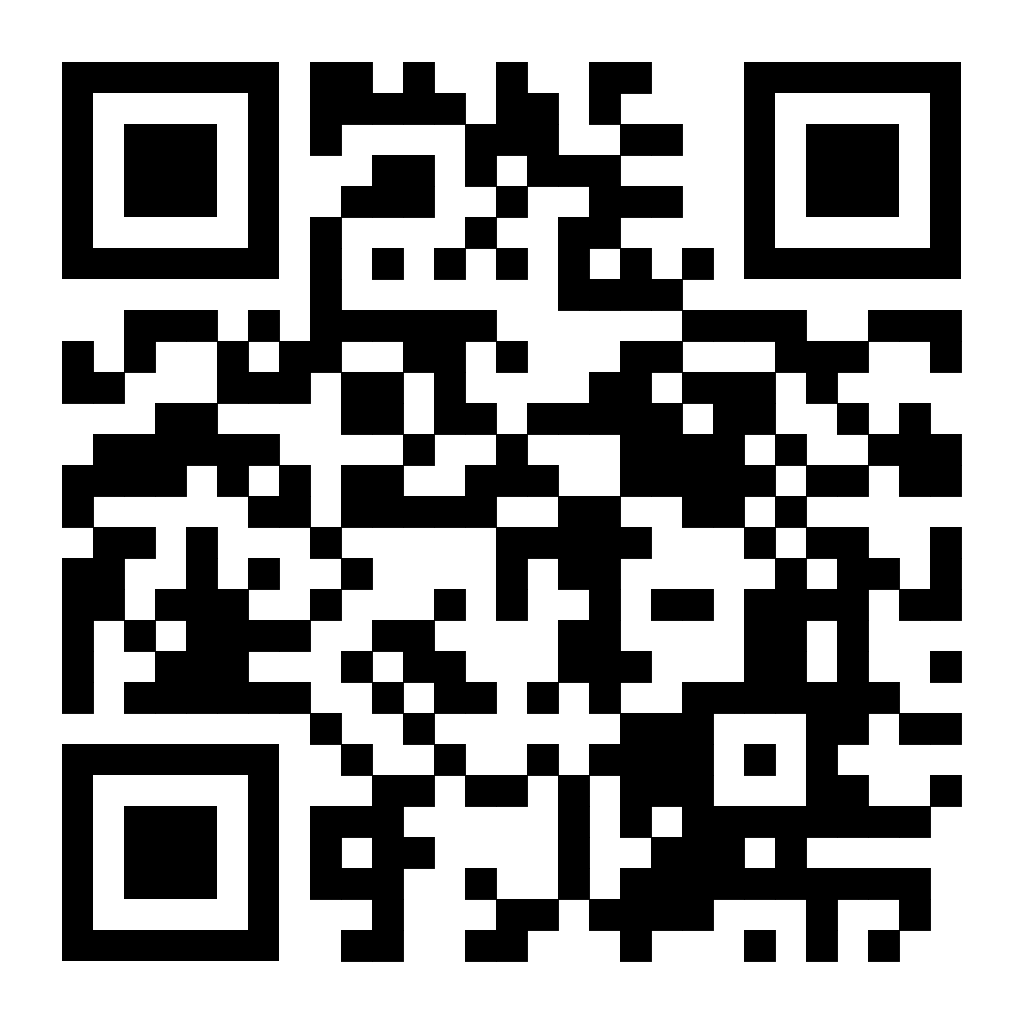
\includegraphics[scale=0.05]{imgs/algebraic.png}};
	    \draw[,->,thick] (link) to [in=180,out=-90] (qr.west);
	 \end{tikzpicture}
	\vfill
\end{frame}

\setLayout{mainpoint}
\begin{frame}[noframenumbering,plain]{Let's see some results} 
\end{frame}

\setLayout{vertical}
\begin{frame}[noframenumbering,plain]{Analysis of the coined quantum walks} 
    \vfill 
    \centering
        \pgfplotstableread{codes/coined_walk.dat}{\table}
         
        \begin{tikzpicture}\centering
            \begin{axis}[
                xmin = 1, xmax = 11,
                ymin = 0, ymax = 900,
                xtick distance = 1,
                ytick distance = 200,
                grid = both,
                minor tick num = 1,
                major grid style = {lightgray},
                minor grid style = {lightgray!25},
                width = \textwidth,
                height = 0.5\textwidth,
                legend cell align = {left},
                legend pos = north west,
                legend style={nodes={scale=0.7, transform shape}}, 
                %legend image post style={mark=*},
                xlabel={$n_1$},
                ylabel={$\dim(\cdot)$}
            ]
             
            %\addplot[NavyBlue, mark = *, dashed] table [x = {x}, y = {y1}] {\table};
             
            \addplot[orange, mark = *, dashed] table [x ={x}, y = {y2}] {\table};
             
            \addplot[ForestGreen, mark = *, dashed] table [x = {x}, y = {y3}] {\table};
            
            \addplot[red, mark = *, dashed] table [x ={x}, y = {y4}] {\table};
             
            \legend{
                %$\dim(\mathscr{N}^\perp)$ - random, 
                $\dim(\mathscr{N}^\perp)$ - reflection coin,
                $\dim(\mathscr{N}^\perp)$ - Hadamard coin,
                $\dim(\hH)$
            }
             
            \end{axis}
         
        \end{tikzpicture}
    \vfill
    \end{frame}

    \setBGColor{c2}
    \setLayout{blank}
    \begin{frame}[noframenumbering,plain]{Imported code from file}
        \vfill
        \vspace{-0.5cm}
        \begin{columns}
        \column{0.5\textwidth}
        {\color{black}
        \begin{align*}
            G(s) &= \frac{5s+50}{s^2+101s+100}\\ 
            &= 5\frac{s+10}{(s+1)(s+100)}
        \end{align*}

        \bigskip
        $$ \begin{cases}\dot{x}(t) = Ax(t) + Bu(t)\\
        y(t) = Cx(t) + D u(t)
        \end{cases}$$
        \begin{align*}
            &A=\begin{bmatrix}0&1\\-100&-101\end{bmatrix}, 
        \quad &B =\begin{bmatrix}0\\1\end{bmatrix}, \\
        \quad &C =\begin{bmatrix}50&5\end{bmatrix}, 
        \quad &D =\begin{bmatrix}0\end{bmatrix}
        \end{align*}}
        \column{0.5\textwidth}
        \codesection{}{codes/slide1.m}

        \end{columns}
        \vfill
    \end{frame}

    \setLayout{vertical}
    \begin{frame}[noframenumbering,plain,fragile]{Inline code (Clearly needs some work)}
        \vfill
        \hspace{-2cm}
        \begin{columns}
        \column{0.5\textwidth}
        \vspace{-0cm}
        \hspace{-1cm}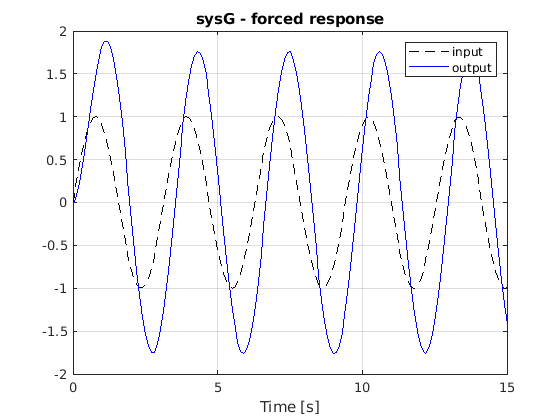
\includegraphics[scale=0.5]{forced.png}
        \column{0.5\textwidth}
        \vspace{-6cm}\hspace{-2cm}
        \begin{code}{Display forced response}
        t = 0:0.1:15;  
        u = sin(2*t);   
        x0 = 0;         
        y = lsim(sysG, u, t, x0);
        
        figure;
        plot(t, u, 'k--');
        hold on;
        plot(t, y, 'b');
        legend('input', 'output');
        grid on;
        \end{code}
        \end{columns}
        \vfill
    \end{frame}

    \begin{frame}[noframenumbering,plain]{Columns}
        \vfill
        \bigskip
        \begin{columns}
        \column{0.4\textwidth}
        \alert{Encapsulated form:}\\
        The CST stores and uses the model-related data via LTI objects (objects in the sense of object-oriented programming). 
        \column{0.5\textwidth}
        \alert{Non-encapsulated form:}\\
        poles and zeros, state/input/output matrices etc. etc.
        \end{columns}
        \bigskip
        From the encapsulated form it is possible to access the non-encapsulated data via dot-notation

    \vfill
    \end{frame}

%------------------------------------CONCLUSION--------------------------------------------
\setBGColor{UNIPDred}

\setBGColor{UNIPDred}
\setLayout{vertical}
\begin{frame}[noframenumbering,plain]{Conclusions and outlook} 
\vfill 
Classical control tools can be used to study quantum walks and find the minimal linear model capable of reproducing the output probability distribution.

Grover's algorithm uses surprisingly few resources.\bigskip

Future directions:
\begin{itemize}
    \item Robustness to initialization errors. 
    \item More general output functions. 
    \item \textbf{\color{UNIPDred}Completely positive and trace preserving constraint.}
\end{itemize}

\vfill
\end{frame}


\setLayout{blank}
\begin{frame}[noframenumbering,plain]
	\centering
	
	\vspace{1cm}
	\textbf{\Huge Thank you for your attention!} 
	
	\vspace{1cm}
	\tikzmark{qr}{
\includegraphics[scale=0.05]{imgs/my_website.png}}
 	\begin{tikzpicture}[overlay, remember picture,node distance =.8cm]
	    \node(word) at (-4,0) {My website};
% 	    \node(qr) at (0,0) {};
 	    \draw[,->,thick] (word.east) to [in=180,out=45] (qr.west);
 	 \end{tikzpicture}
	
	\vspace{1cm}
	
	\begin{figure}
		\centering
		\begin{subfigure}{0.2\textwidth}
			\centering
			
\includegraphics[height=2cm]{lib/logos/dei_white.png}
		\end{subfigure}
	\hspace{1cm}
	\vrule \ \hspace{1cm}
		\begin{subfigure}{0.2\textwidth}
			\centering
			
\includegraphics[height=2cm]{lib/logos/unipd_white.png}
		\end{subfigure}
		
	\end{figure}
\end{frame}

\end{document}